\begin{center}
\textbf{МНОГОКРАТНЫЕ ПРЯМЫЕ ИЗМЕРЕНИЯ ФИЗИЧЕСКИХ 
ВЕЛИЧИН И ОБРАБОТКА РЕЗУЛЬТАТОВ НАБЛЮДЕНИЙ}

\vspace{1.0cm}

\section{\textbf{Введение}}
\end{center}

Основными задачами лабораторной работы являются: \\
\indent1. Освоить методику использования измерительного прибора для 
многократного прямого измерения физической величины.\\
\indent2. Выполнить простейшую статистическую обработку серии 
результатов наблюдений при прямых измерениях.

\vspace{0.5cm}

\begin{center}
Установка
\end{center}

\begin{figure}[H]
\centering

\includegraphics[width=0.9\textwidth]{image.png}
\caption{Установка}
\label{fig:distribution}
\end{figure}

Вычисление погрешности прибора \(\Delta T_{\text{прибл}}\):
\[\Delta T_{\text{прибл}} = \gamma_T \cdot T_{\text{ср}}\]

\[\gamma_T = \pm \left(\gamma_0 + \frac{T_0}{T_{\text{ср}}}\right) = \frac{\Delta T_{\text{прибл}}}{T_{\text{ср}}}, \quad T_{\text{ср}} = \frac{\sum_{i=1}^n T_i}{n}\]

где: \(\gamma_T\) -- относительная погрешность измерения, \(\gamma_0 = 5 \cdot 10^{-7}\), \(T_0 = 10^{-4}\) c \\
для грубых измерений (\(n = 10\)), \(T_0 = 10^{-6}\) c для точных измерений (\(n = 50\)).

\begin{center}
\section{Таблицы}
\end{center}

\noindent\textbf{1. Грубые измерения.}

\vspace{0.3cm}

{\centering
\captionof{table}{Измерения на грубой шкале}
\label{tabl:1}
\begin{tabular}{|c|c|c|c|c|}
\hline
\begin{minipage}{7mm}
    № п.п. 
\end{minipage}&
\begin{minipage}{5cm}
    Диапазон показаний использованной шкалы прибора
\end{minipage} &
\begin{minipage}{5cm}
    Результаты отдельных наблюдений ($T_i$)
\end{minipage} &
\begin{minipage}{5cm}
    Погрешность прибора на данной шкале ($\Delta T_{\text{приб}}$)
\end{minipage}\\
\hline
{}&мс&мс&мс\\
\hline
1 & 0-10\(^6\) & 273.8 & 0.1 \\
2 & 0-10\(^6\) & 274.0 & 0.1 \\
3 & 0-10\(^6\) & 273.8 & 0.1 \\
4 & 0-10\(^6\) & 273.8 & 0.1 \\
5 & 0-10\(^6\) & 273.6 & 0.1 \\
6 & 0-10\(^6\) & 273.7 & 0.1 \\
7 & 0-10\(^6\) & 273.1 & 0.1 \\
8 & 0-10\(^6\) & 273.3 & 0.1 \\
9 & 0-10\(^6\) & 273.1 & 0.1 \\
10& 0-10\(^6\) & 273.4 & 0.1 \\
\hline
\end{tabular}
\par} 

\FloatBarrier 

\vspace{0.5cm}
\noindent \(\overline{T} = 273.66\) мс, \(\Delta T_{\text{приб}} = 0.1\) мс

\vspace{0.5cm}
\noindent\textbf{2. Точные измерения.}\\

\vspace{0.3}

Перейдем на более точную шкалу и измерим 50 величин для получения выборки:
\\

диапазон показаний прибора 0-10\(^4\) мс
\\

погрешность прибора по формуле выше $\Delta T_{\text{приб}}$=\pm 0.00114 мс

\vspace{0.5cm}
\begin{longtable}{|c|p{3.2cm}|p{3.5cm}|p{3.5cm}|}
\caption{Измерения на точной шкале}
\label{tabl:2}\\
\hline
\textbf{Номер п.п.} & \textbf{Результаты отдельных наблюдений ($T_i$)} & \textbf{Случайные отклонения от среднего $d_i = T_i - \overline{T}$} & \textbf{$d_i^2 = (T_i - \overline{T})^2$} \\
\hline
 & \textbf{(мс)} & \textbf{(мс)} & \textbf{(мс\(^2\))} \\
\hline
\endfirsthead

\hline
\textbf{Номер п.п.} & \textbf{Результаты отдельных наблюдений ($T_i$)} & \textbf{Случайные отклонения от среднего $d_i = T_i - \overline{T}$} & \textbf{$d_i^2 = (T_i - \overline{T})^2$} \\
\hline
 & \textbf{(мс)} & \textbf{(мс)} & \textbf{(мс\(^2\))} \\
\hline
\endhead

\hline
\multicolumn{4}{|r|}{Продолжение на следующей странице} \\
\endfoot

\hline
\endlastfoot

1  & 274.414 & 0.4583 & 0.2100 \\
2  & 274.576 & 0.6203 & 0.3848 \\
3  & 274.321 & 0.3653 & 0.1334 \\
4  & 274.064 & 0.1083 & 0.0117 \\
5  & 274.535 & 0.5793 & 0.3356 \\
6  & 273.976 & 0.0203 & 0.0004 \\
7  & 273.694 & -0.2617 & 0.0685 \\
8  & 273.821 & -0.1347 & 0.0181 \\
9  & 273.784 & -0.1717 & 0.0295 \\
10 & 273.993 & 0.0373 & 0.0014 \\
11 & 273.358 & -0.5977 & 0.3572 \\
12 & 273.466 & -0.4897 & 0.2398 \\
13 & 274.188 & 0.2323 & 0.0540 \\
14 & 274.120 & 0.1643 & 0.0270 \\
15 & 274.151 & 0.1953 & 0.0381 \\
16 & 274.366 & 0.4103 & 0.1683 \\
17 & 274.267 & 0.3113 & 0.0969 \\
18 & 274.019 & 0.0633 & 0.0040 \\
19 & 274.118 & 0.1623 & 0.0263 \\
20 & 273.799 & -0.1567 & 0.0246 \\
21 & 273.800 & -0.1557 & 0.0242 \\
22 & 273.931 & -0.0247 & 0.0006 \\
23 & 273.866 & -0.0897 & 0.0080 \\
24 & 274.101 & 0.1453 & 0.0211 \\
25 & 274.062 & 0.1063 & 0.0113 \\
26 & 273.834 & -0.1217 & 0.0148 \\
27 & 273.917 & -0.0387 & 0.0015 \\
28 & 274.297 & 0.3413 & 0.1165 \\
29 & 274.151 & 0.1953 & 0.0381 \\
30 & 274.252 & 0.2963 & 0.0878 \\
31 & 273.511 & -0.4447 & 0.1978 \\
32 & 273.556 & -0.3997 & 0.1598 \\
33 & 273.831 & -0.1247 & 0.0156 \\
34 & 273.597 & -0.3587 & 0.1287 \\
35 & 273.482 & -0.4737 & 0.2244 \\
36 & 274.076 & 0.1203 & 0.0145 \\
37 & 273.932 & -0.0237 & 0.0006 \\
38 & 273.965 & 0.0093 & 0.0001 \\
39 & 273.929 & -0.0267 & 0.0007 \\
40 & 273.933 & -0.0227 & 0.0005 \\
41 & 273.664 & -0.2917 & 0.0851 \\
42 & 273.917 & -0.0387 & 0.0015 \\
43 & 274.127 & 0.1713 & 0.0293 \\
44 & 274.018 & 0.0623 & 0.0039 \\
45 & 274.089 & 0.1333 & 0.0178 \\
46 & 273.571 & -0.3847 & 0.1480 \\
47 & 273.791 & -0.1647 & 0.0271 \\
48 & 273.330 & -0.6257 & 0.3915 \\
49 & 273.808 & -0.1477 & 0.0218 \\
50 & 273.366 & -0.5897 & 0.3477 \\
\hline
\multicolumn{1}{|c|}{} & \textbf{\(\overline{T} = \frac{\sum T_i}{50} = 273.956\)} & \textbf{\(\sum |d_i| = 13.427\)} & \textbf{\(\sum d_i^2 = 4.828\)} \\
\hline
\end{longtable}

\begin{figure}[H]
\centering
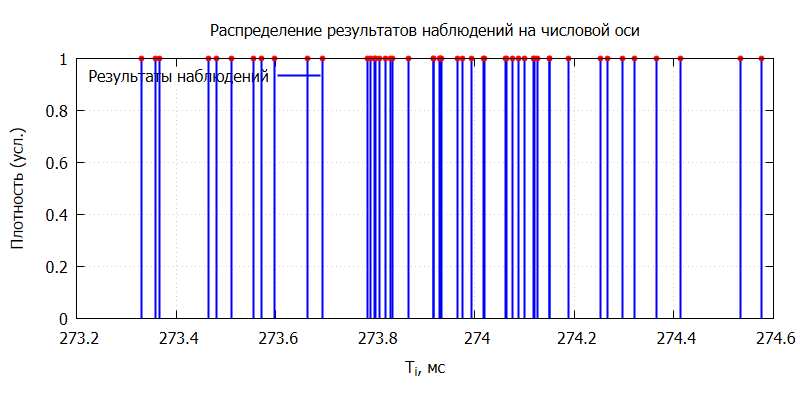
\includegraphics[width=0.9\textwidth]{distribution_stem.png}
\caption{Распределение результатов наблюдений на числовой оси}
\label{fig:distribution}
\end{figure}

\[ T_{\min} = 273.330 \, \text{мс}, \quad T_{\max} = 274.576 \, \text{мс} \]

\begin{table}[ht!]
\centering
\caption{Распределение результатов наблюдений по интервалам}
\label{tab:distribution}
\begin{tabular}{|c|c|c|c|}
\hline
\textbf{Номер интервала} & \textbf{Границы интервала} & \textbf{Число случаев (\(\Delta n\))} & \textbf{\(\delta n = \frac{\Delta n}{n}\)} \\
\hline
 & ширина 0,15мс & \(\sum \Delta n = 50\) & \(\sum \frac{\Delta n}{n} = 1\) \\
\hline
1 & [273.30, 273.45) & 5 & 0.10 \\
2 & [273.45, 273.60) & 5 & 0.10 \\
3 & [273.60, 273.75) & 4 & 0.08 \\
4 & [273.75, 273.90) & 11 & 0.22 \\
5 & [273.90, 274.05) & 9 & 0.18 \\
6 & [274.05, 274.20) & 9 & 0.18 \\
7 & [274.20, 274.35) & 4 & 0.08 \\
8 & [274.35, 274.50) & 2 & 0.04 \\
9 & [274.50, 274.65) & 1 & 0.02 \\
\hline
\end{tabular}
\end{table}

Рассчитаем стандартное отклонение по формуле:
\[
\sigma \approx \sqrt{\frac{1}{n-1} \sum_{i=1}^{n} (x_i - \overline{x})^2}
\]

Подставляя наши данные (\(n = 50\), \(\sum d_i^2 = 4.828\)):
\[
\sigma \approx \sqrt{\frac{4.828}{49}} = \sqrt{0.09853} \approx 0.314\ \text{мс}
\]

Полученное значение \(\sigma \approx 0.314\) мс характеризует случайный разброс результатов измерений относительно среднего.
\\
\\

Средняя квадратичная погрешность среднего:
\[
\Delta T \approx \frac{\sigma}{\sqrt{n}} = \frac{0.314}{\sqrt{50}} = \frac{0.314}{7.071} \approx 0.0444\ \text{мс}
\]

Окончательный результат:
\[
T = \overline{T} \pm \Delta T = 273.956 \pm 0.044\ \text{мс}
\]

\begin{center}
\section{Графики}
\end{center}


\begin{figure}[H]
\centering
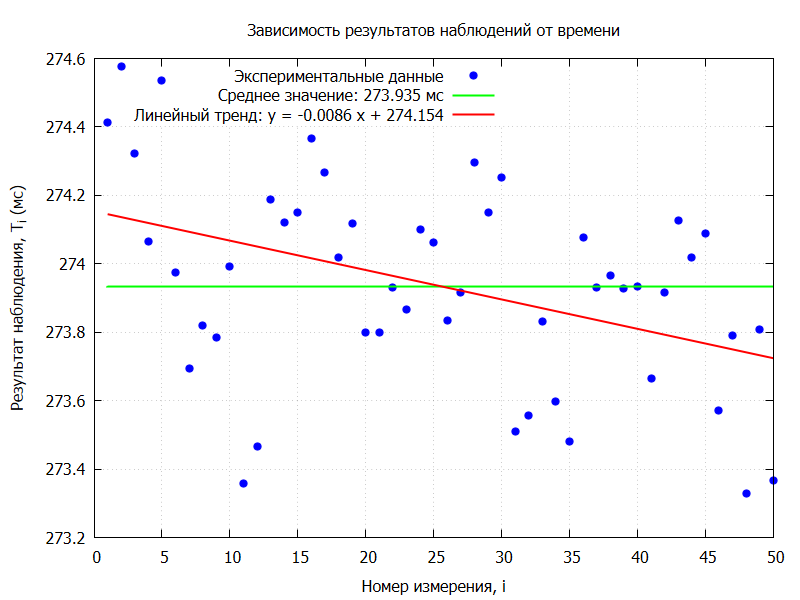
\includegraphics[width=0.8\textwidth]{drift_plot_with_mean.png}
\caption{Зависимость результатов наблюдений от времени}
\label{fig:drift}
\end{figure}

\begin{figure}[H]
\centering
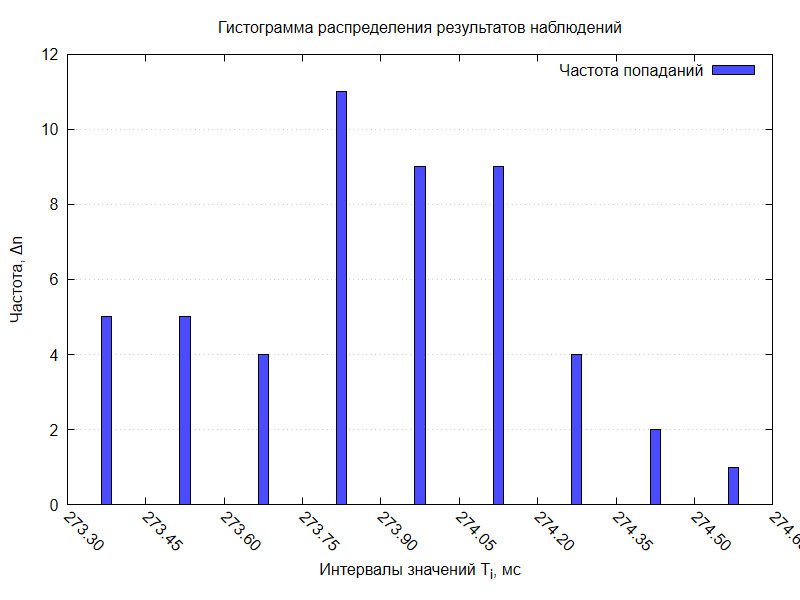
\includegraphics[width=0.9\textwidth]{histogram_fixed.png}
\caption{Гистограмма распределения результатов наблюдений}
\label{fig:histogram}
\end{figure}

\section{Выводы}
В результате проделанной работы я познакомился с методиками использования измерительного прибора для многократного прямого измерения физической величины на примере работы с электронным частотомером Ч3-32, научился выполнять простую статистическую обработку серии результатов наблюдений при прямых измерениях (с вычислением дисперсии и среднеквадратичным отклонением).